\section{Biological Background}
\centering
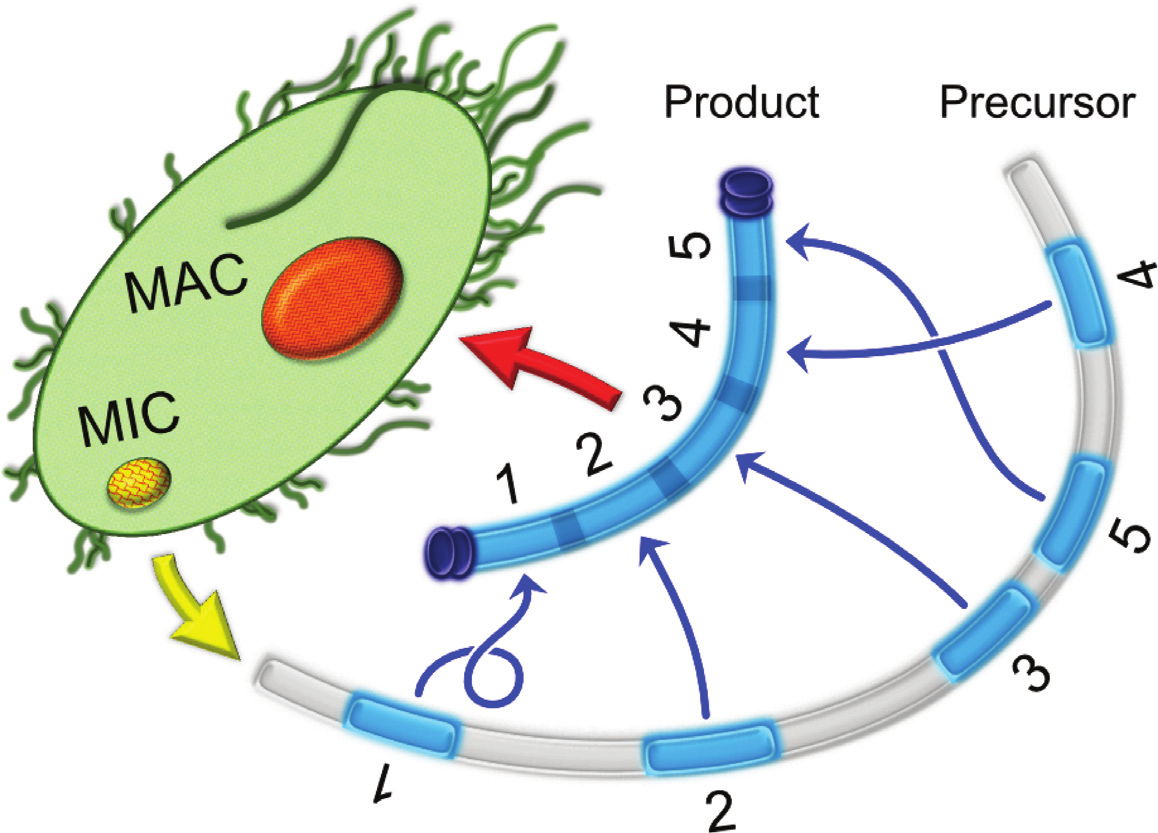
\includegraphics[width=250px]{0}

The ciliate Oxytricha is a microbial eukaryote with two genomes, one of which experiences
extensive genome remodeling during development. Each round of conjugation initiates a cascade
of events that construct a transcriptionally active somatic genome from a scrambled germline
genome, with considerable help from both long and small noncoding RNAs. This process of


\section{Formalisation}
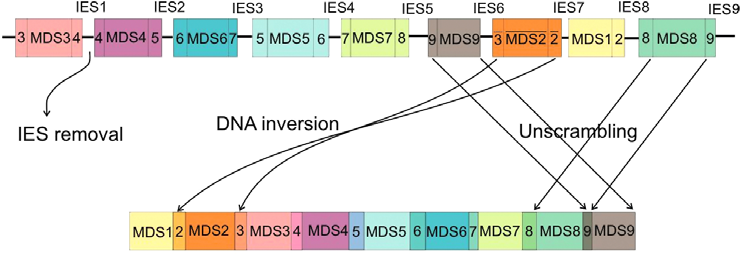
\includegraphics[width=\textwidth]{1}

\section{Existent Approaches/Solutions}

\section{ILP formulation}